%% ----- INTRODUCTION -----
\hypertarget{server-experiments-introduction}{%
\section{Introduction}\label{server-experiments-intro}}

Before my arrival at VSP in Berlin, I amassed two decades of software development experience, almost entirely at the intersection of transport modelling and user interface design. This unusual combination led to some interesting and novel research, such as the CycleTracks bicycle route choice model and mobile-phone based data collection approach in \cite{HoodSallCharlton2011BicycleRouteChoiceSanFrancisco}, the QuickMuni transit-arrival app\footnote{QuickMuni, available at \url{https://play.google.com/store/apps/details?id=com.worldofbilly.quickmuni}}, and the San Francisco County Transportation Authority "TNCs Today" data exploration web portal in \cite{erhardt2019transportation}.

The interest at VSP in developing web-based visualizations for MATSim outputs was high, so we set out to adapt some of the technologies used in the efforts listed above. Initially there was no end-goal in mind; these were pure research to see how far we could go with web-based technologies. Given the recent improvements in HTML 5 and JavaScript, we were unsure just how far we could go.

This chapter describes several of these initial experiments and the findings thereof.

The first experiment is a web-based MATSim transit network viewer, which reads and displays MATSim network and transit schedule files, producing an interactive page allowing the user to explore different public transit routes and lines, including display of summary statistics for selected routes. This tool is entirely client-side JavaScript code.

The second is an accessibility data web portal using a pre-existing GeoServer back-end, which holds the accessibility datasets and geographic boundary files, and a JavaScript web front end allowing the user to explore the datasets for a given area.

Third, a tool to display and explore MATSim emissions outputs is described. This tool pushed the limits of the size of datasets that can be ingested by a desktop web-browser, using various techniques to optimize the display of large datasets without a server back end.

Finally we close this chapter with summary findings about these experiments and where the experiments led us: to a more centralized client/server tool, which is fully described in \autoref{ch:mathub}.

%% ----- TRANSIT VIEWER -----
\hypertarget{server-experiments-transit}{%
\section{MATSim Transit Network Viewer}\label{server-experiments-transit}}

The first step in building web-based tools for MATSim was reading and parsing MATSim input files using JavaScript. MATSim inputs representing the transportation network and public transit supply are both well-defined XML formats YY and are of a size that does not present problems as they can easily be loaded in memory. Based on feedback from team members, a transit service explorer was identified as a good first task.

A minimally-useful tool needed the following capabilities:

\begin{itemize}
  \tightlist
  \item
    Load and parse a MATSim network XML file and transit supply XML file, including gzip-compressed versions of these files, as gzip is typically used to compress MATSim files
  \item
    Display the network links on a zoomable background map
  \item
    Display the transit lines and routes that are on network links, using width and color to depict multiple routes or transit modes on a facility
  \item
    Allow the user to select a facility (link) and see the details of the transit routes and lines which use it
\end{itemize}

The JavaScript ecosystem offers an enormous package of useful libraries in the Node Package Manager, or NPM\footnote{NPM, the Node Package Manager, available at \url{https://npmjs.org}}. It did not take long to find an appropriate XML parser\footnote[1]{fast-xml-parser, available at \url{https://www.npmjs.com/package/fast-xml-parser}} and geospatial mapping library\footnote[2]{MapBox GL, available at \url{https://mapbox.com}} which were used as the starting point for this effort.

\hypertarget{server-experiments-files}{%
\subsection{File storage and local file access via web browser}
\label{server-experiments-files}}

This seemingly small project presented some initial challenges. First and foremost, by design and to protect the security of a user's files, web browsers do not allow any access to the files on a user's local computer. This makes sense when protecting users from malicious websites, but for a local experiment we need to find a way around this. Several solutions exist:

\textbf{Moving files to an HTTP-accessible file server.} At VSP there is already a departmental file server accessible via HTTP, which uses Subversion\footnote{Subversion, available at \url{https://subversion.apache.org/}} and provides both world-readable and password-protected areas for file storage. Files on these servers can be accessed if the user has the URL and the area password (if necessary). For our initial test case, this was the easiest solution.

\textbf{Running a local HTTP server.} It is trivial to run a local (meaning on the user's computer or laptop) HTTP server. A simple HTTP file server is included in every install of the Python programming language, for example, and can be run from the command-line with one command\footnote{For Python 3 the command is "python -m http.server"}. The folder in which the command is run is then accessible at the url \url{http://localhost:8000}, allowing local-only access to those files. This approach will be discussed in much more detail in \autoref{ch:simwrapper}.

\textbf{Building a desktop app instead of a website.} Beyond the scope of this initial experiment is the development of a desktop app instead of a website. Desktop apps do not have the same restrictions as websites, and can be granted full access to the files on a user's computer. There are several frameworks for converting JavaScript-based websites to desktop apps, including Electron and React Native, which were briefly considered but discarded for this test, as we specifically wanted to focus on web-accessible approaches.

For this transit network viewer, both approaches of having the files locally-accessible via the python server, or copying the files to the departmental file server, were sufficient for our needs. This challenge with file storage will come up again and again in the research presented here.

\hypertarget{server-experiments-coords}{%
\subsection{Coordinate systems and coordinate conversion}
\label{server-experiments-coords}}

The only other challenging topic in this initial project is coordinate conversion. MATSim is entirely agnostic about the X/Y coordinates used for its networks. Typically a cartesian system with meters or feet is used, but there is no hard requirement.

Drawing MATSim networks on a background map requires conversion of the coordinates to longitude/latitude, as every major web-based mapping library expects coordinates to be in Earth-based spherical coordinates, often referred to as WGS84 or EPSG:4326. Again there are NPM-based librares to perform this conversion, but it requires the end user to know what coordinate system their networks are stored in.

Recent versions of MATSim since 2019 embed the coordinate reference system in the MATSim configuration files, so this is usually trivial now, but there are scores of older network files that do not have this information stored and require trial-and-error or memory to discover the correct transformation.

\hypertarget{server-experiments-transit-result}{%
\subsection{The transit viewer tool}
\label{server-experiments-tool-transit}}

\autoref{fig:transit-viewer} shows an example usage of the transit network viewer tool. The public transport network of Cottbus, a small city in eastern Germany, is depicted. All streets with local transit are drawn in red, while all transit services using a user-selected link are shown in yellow and green. The specific transit routes on the selected link are also listed in a detailed view in the upper left, describing the first and last departures for the route and the number of runs per day for that route.

Testing confirms that transit networks as large as the entire Berlin region, including all bus and rail passenger transport, are also viewable and performant using the tool.

\begin{figure}[!ht]
  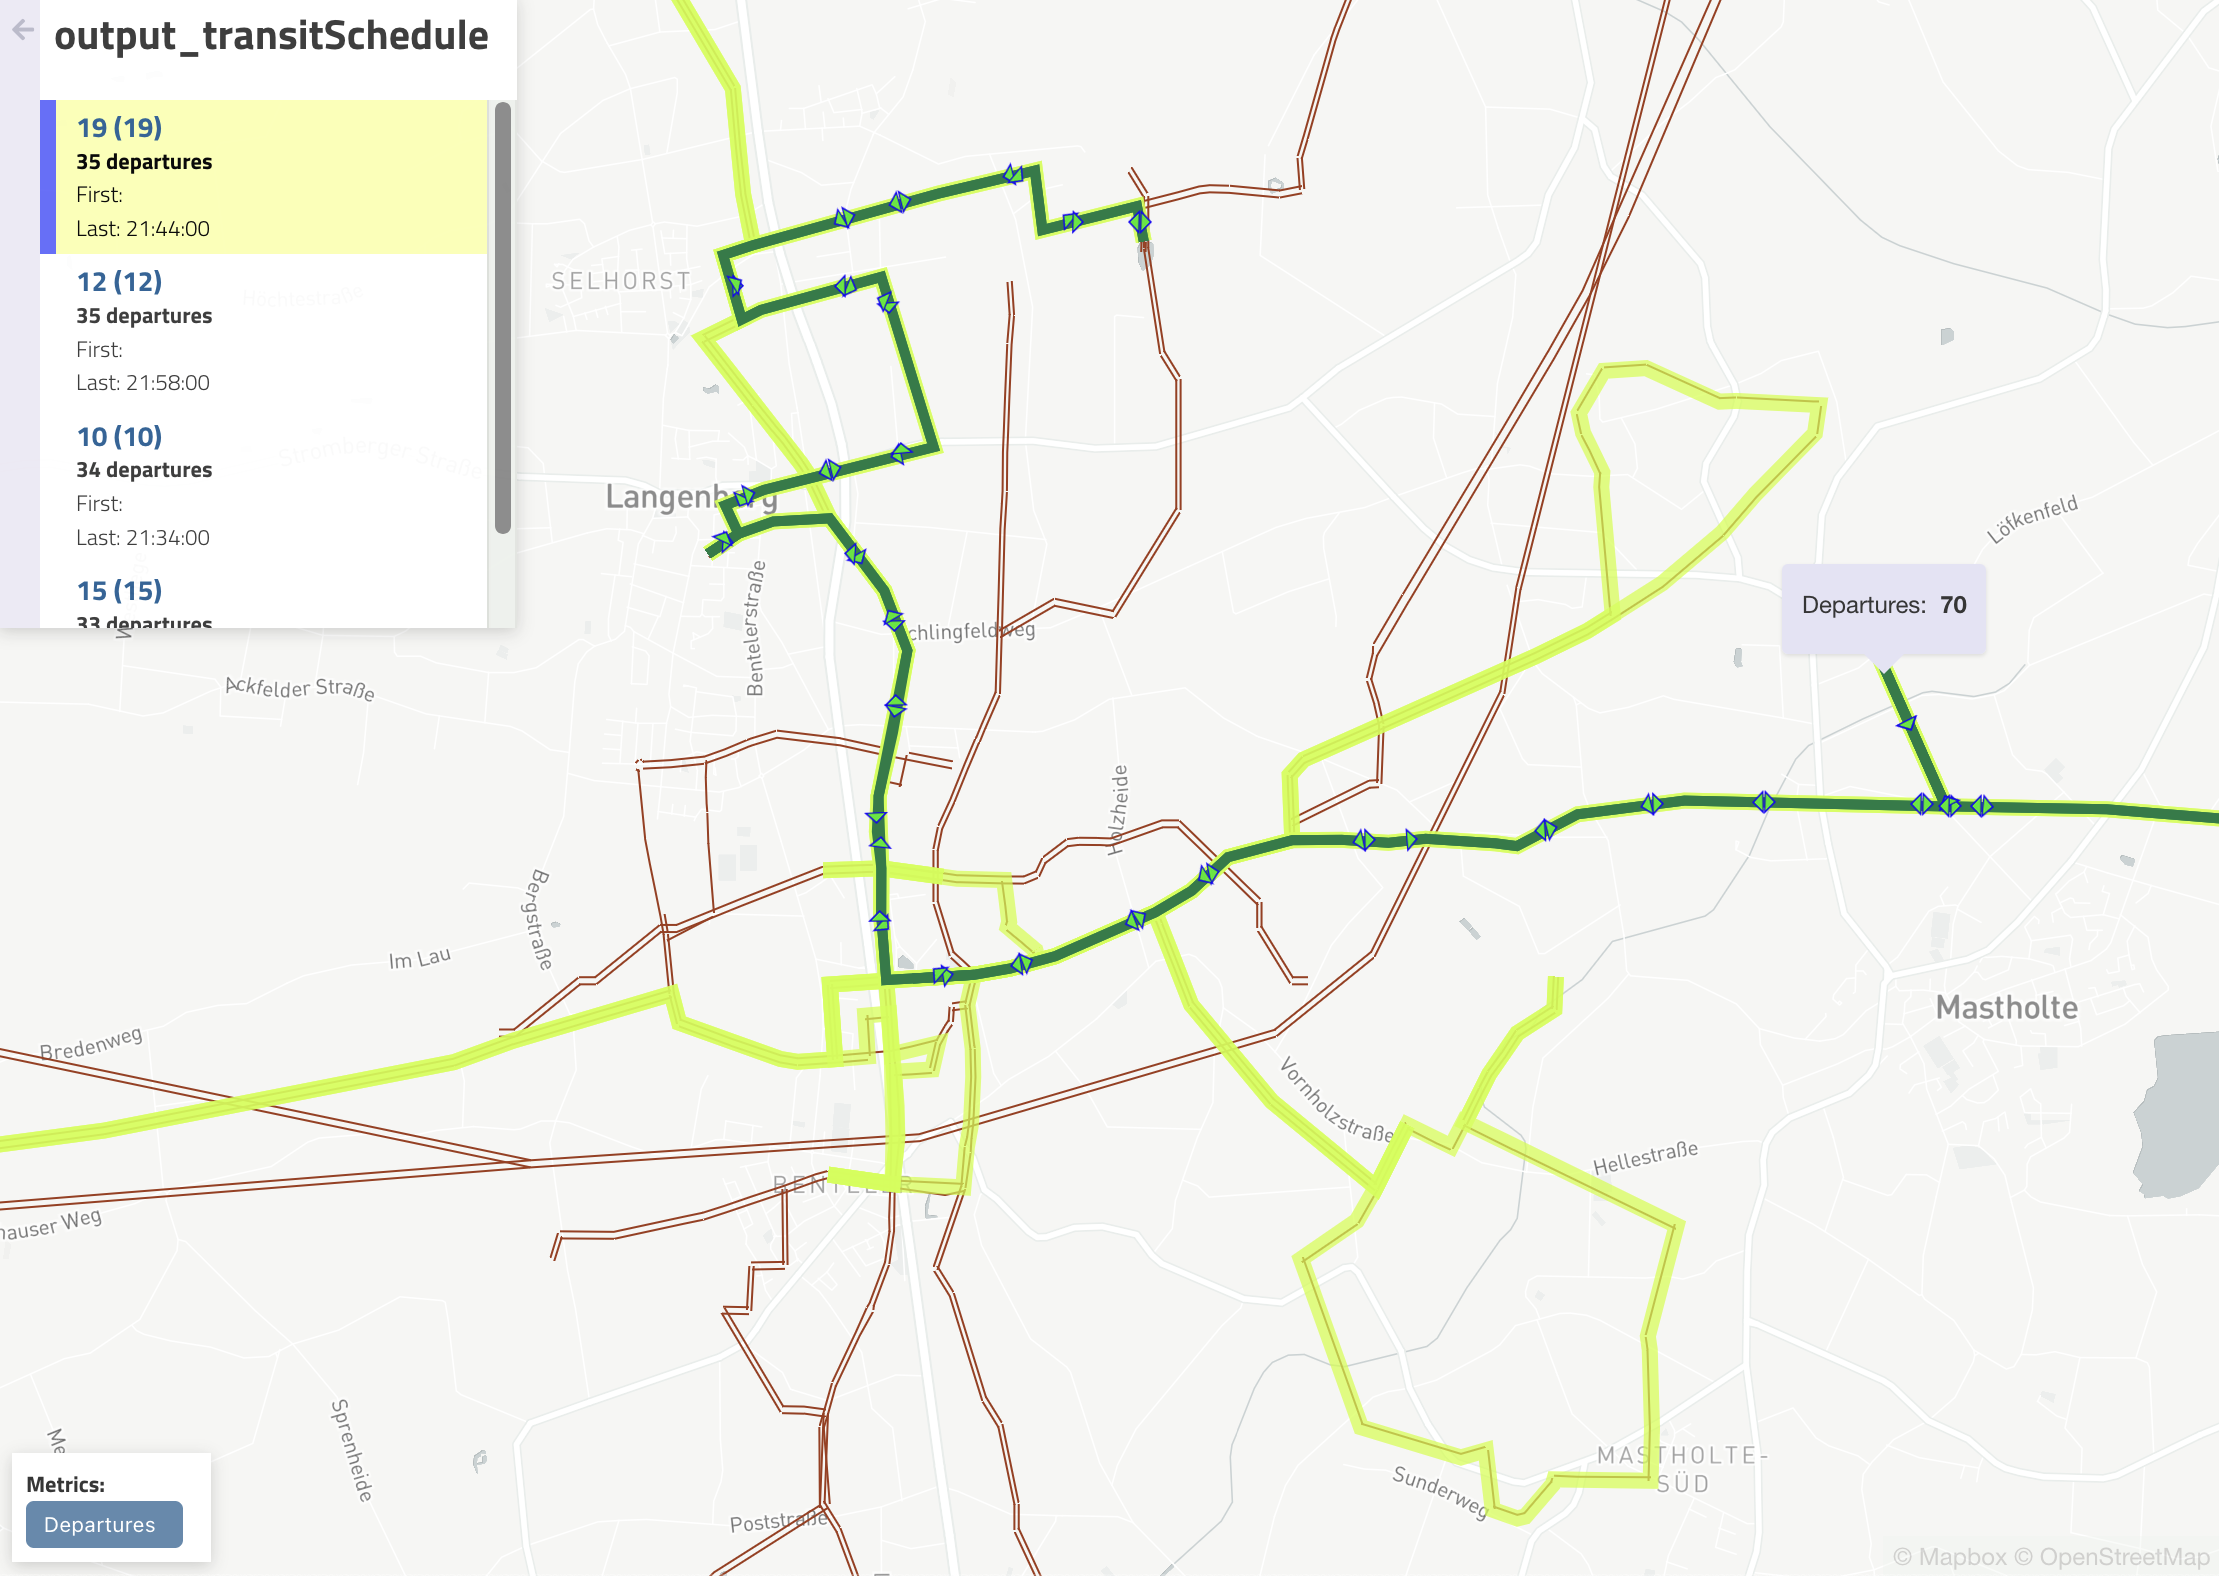
\includegraphics[width=\textwidth]{chapters/01-server-experiments/images/transit-viewer.png.pdf}
  \caption{Web-based transit network viewer. This depicts the public transit network of Cottbus, Germany, a small city in eastern Germany. One central link is selected, with the various transit routes using that line highlighted in yellow and green.}
  \label{fig:transit-viewer}
\end{figure}

As the user highlights routes in the detail view, or selects different road facilities on the map, the colors and details update immediately, allowing the user to explore the network in an interactive way.

Users provided positive feedback on the tool, saying that it helped them debug network errors in complex networks. Constructive/negative feedback highlighted initial confusion around file management and coordinate systems.

%% ----- GEOSERVER -----
\hypertarget{server-experiments-geoserver}{%
\section{Accessibility calculations using GeoServer and MATSim}\label{server-experiments-geoserver}}

MATSim can be used to calculate general accessibility measures, as described in \cite{ziemke2018accessibility}. For a project in Nairobi, Kenya, MATSim was used to generate accessibility measures for several different metrics such as access to drinking water, public school locations, and commercial opportunities. For each measure there were multiple scenarios such as current conditions, system breakdowns (such as a contaminated water source) and so on. The proliferation of combinations of measures and scenarios led to the idea of using the a server back-end to store results, along with a web-based front end to review results.

GeoServer, as described in \cite{giannecchini2013geoserver}, is

\begin{displayquote}
\emph{"an Open Source application for the handling and dissemination of geospatial data. GeoServer provides the basic functionalities to create interoperable Spatial Data Infrastructure according to standards edited by the Open Geospatial Consortium (OGC)... GeoServer [can] ingest, manage, and serve both vector and raster geospatial data."}
\end{displayquote}

VSP has an internal GeoServer installation, and the outputs of the accessibility calculations can be uploaded to it easily. Thus for this experiment, instead of a client-side only JavaScript web application, we built a website front end that accessed the data on GeoServer using the GeoServer API.

\hypertarget{server-experiments-geoserver-2}{%
\subsection{Specifying the available accessibility measures using YAML}
\label{server-experiments-geoserver-2}}

GeoServer uses a long "string-id" to identify datasets, e.g. the Kibera, Kenya OSM Live scenario, for drinking water within 50 meters, with a specific color scale for relative differences of 0.5-3.5 units compared to the base case, has a string ID of

\emph{accessibilities:ke\_kibera\_osm\_live\_50\_drinking\_water\_walk\_0.5\_3.5}.

Obviously this is quite unreadable for website text, so the client website reads a YAML-based configuration file which maps the many run configurations to the appropriate GeoServer IDs. The various options are then exposed in the website user interface as drop-down selections, buttons, and so forth.

YAML is a simple text format which uses indentation and punctuation to define and group pairs of key:value configuration data. For example, \autoref{fig:geoserver-yaml} shows a snippet of a YAML configuration for drinking water in Kibera, Kenya.

\begin{figure}[!ht]
  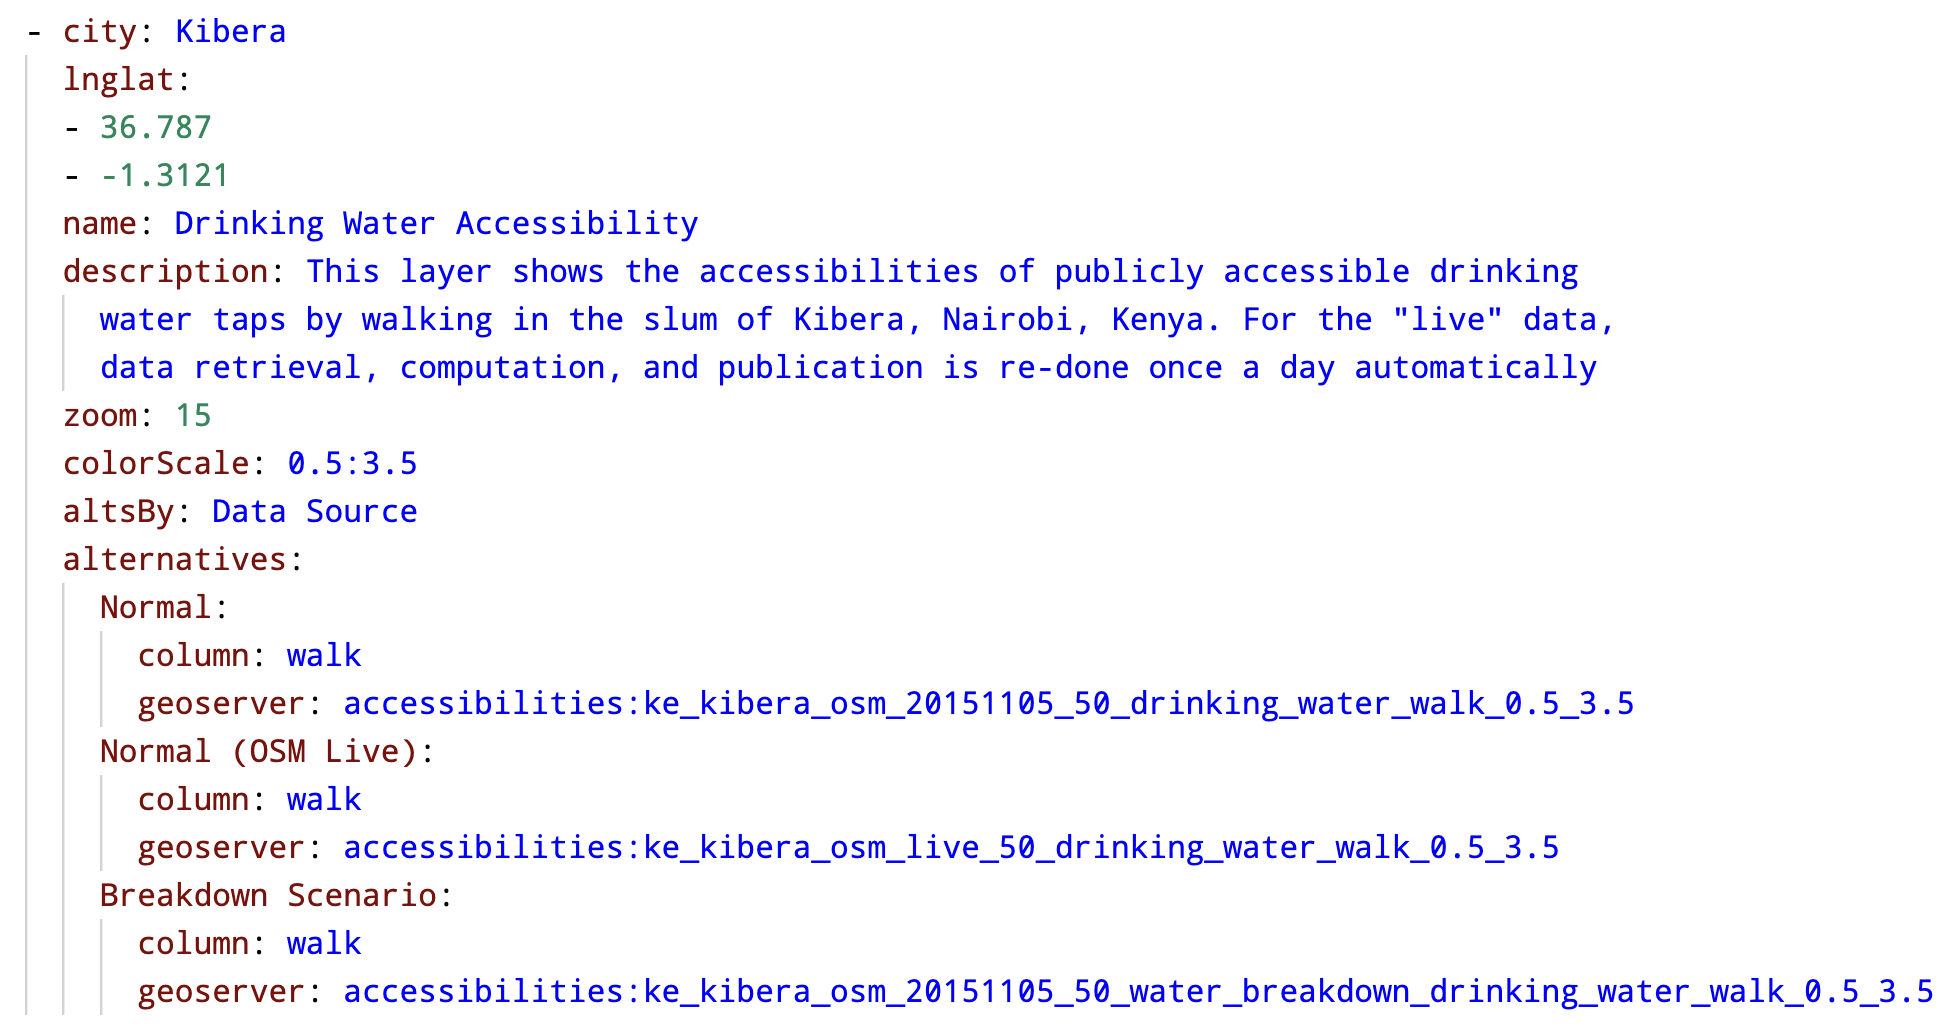
\includegraphics[width=\textwidth]{chapters/01-server-experiments/images/geoserver-yaml.png.pdf}
  \caption{Snippet of YAML configuration which maps user-intelligible information to GeoServer dataset IDs.}
  \label{fig:geoserver-yaml}
\end{figure}

This configuration information when the site is loaded. All of the runs defined in YAML can then be found in the user interface by selecting the metric from a dropdown and choosing the scenario for that metric with a set of buttons. The accessibility data is then pulled from the GeoServer API and displayed on top of the background map.

\hypertarget{server-experiments-geoserver-3}{%
\subsection{The Nairobi, Kenya accessibility data website}
\label{server-experiments-geoserver-3}}

\autoref{fig:nairobi} shows a typical accessibility measure displayed in the website built for the Nairobi, Kenya project. In this image, the selected metric (access to drinking water) and the scenario (normal conditions) are visible, and the grid-based accessibility values calculated by MATSim are plotted on top of the basemap. Hovering over a colored area shows the exact values for the cell in a popup hover window.

\begin{figure}[!ht]
  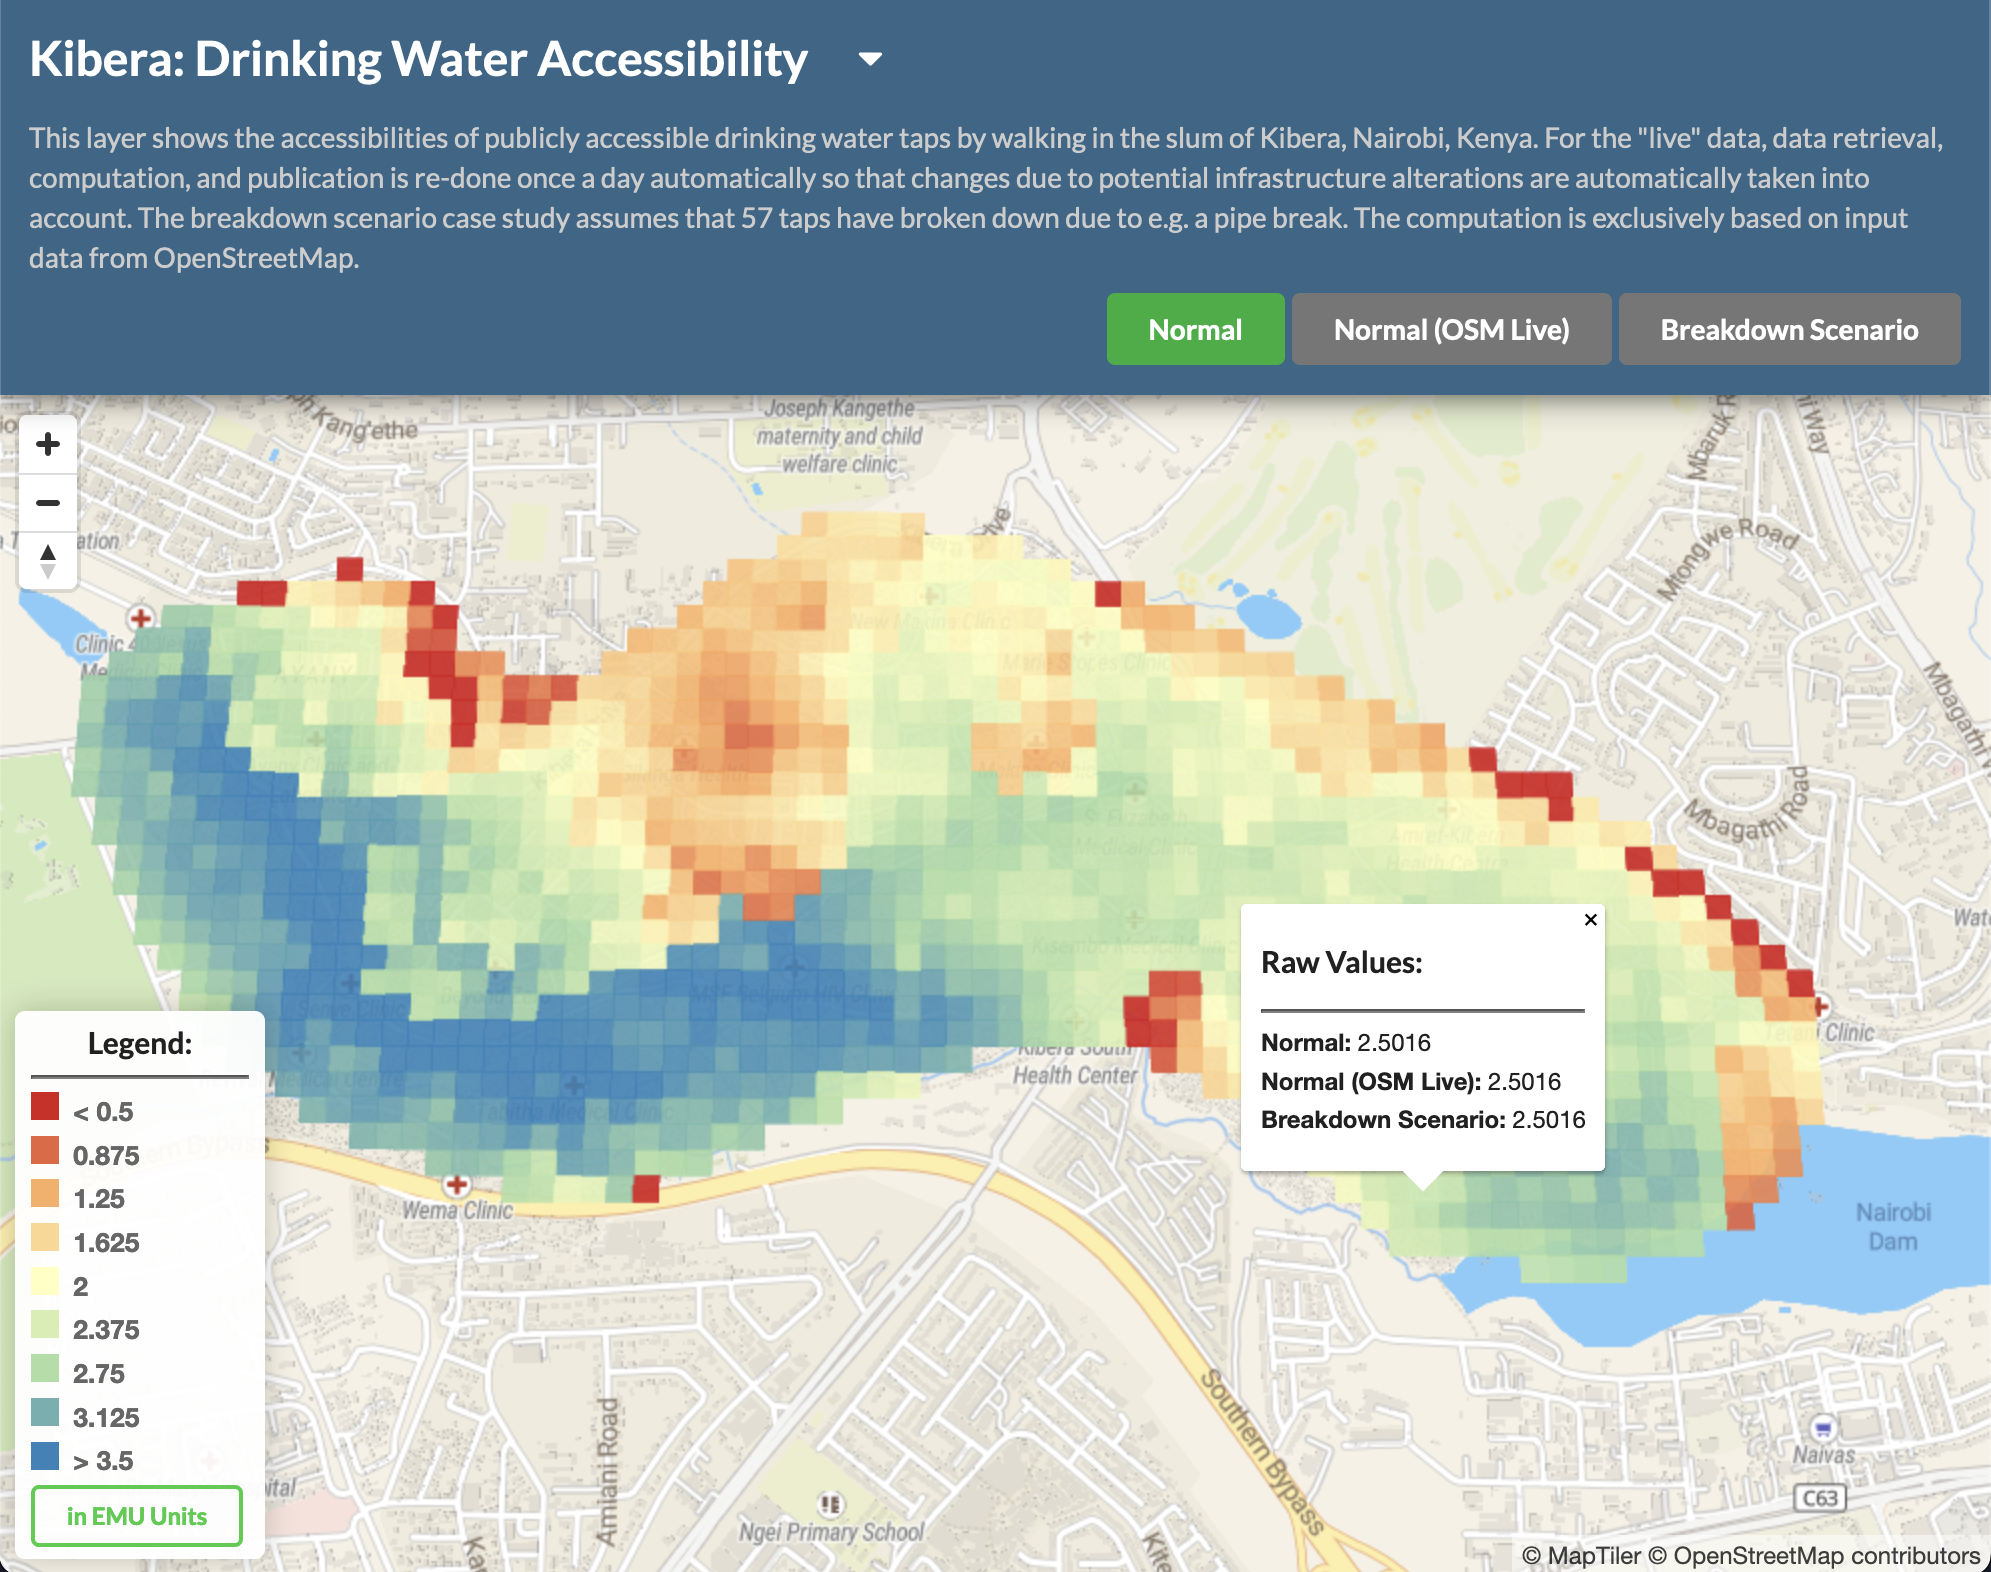
\includegraphics[width=\textwidth]{chapters/01-server-experiments/images/nairobi.png.pdf}
  \caption{Drinking water accessibility calculations, generated by MATSim. This interactive tool allowed users to compare accessibility calculations for drinking water, school locations, and commercial opportunities across several alternatives.}
  \label{fig:nairobi}
\end{figure}

Feedback from internal users was quite positive, as they were able to upload new runs to the server in their usual workflow, and updating the website only required the editing of one configuration file.

This approach required manual updates from the web development team every time new data was available, however. For larger teams or more rapid analysis, a more streamlined and automated approach would be beneficial.

The accessibility website was not developed further after this initial project. Indeed, the GeoServer implementation has not been used for any other purposes since this accessibility research concluded. Interviews revealed that department staff were unclear on the benefits of uploading their datasets to the GeoServer, when they could make non-interactive maps in traditional GIS desktop software, suitable for inclusion in publishable research papers.

%% ----- EMISSIONS  -----
\hypertarget{server-experiments-emissions}{%
\section{MATSim Emissions}\label{server-experiments-emissions}}

%% ----- DISCUSSION AND OUTLOOK  -----
\hypertarget{server-experiments-findings}{%
\section{Discussion and Outlook}\label{server-experiments-findings}}

%% ----- SUMMARY  -----
\hypertarget{server-experiments-summary}{%
\section{Summary}\label{server-experiments-summary}}


Internal use of tools was very limited because of lack of features (could do it all in QGis or VIA); and also because the individual tools were haphazard in their installation. Each one had a separate URL, or required files to be uploaded somewhere users were unaccustomed to.

Through many discussions we decided that the experiments had been useful in pointing us toward building a centralized data analysis platform.

- Show progression from PHD seminar slides

- This led to MatHub: a fully centralized, client/server based approach to creating standard data visualizations.

Next chapter describes that platform fully.


